\begin{frame}{Agenda}
\begin{itemize}
    \item Introduction
    \item Literature Review
    \item Methodology
    \item \textbf{Results}
    \item Conclusion and Future Work
\end{itemize}
\end{frame}

%%

\begin{frame}{Results - \fullNameExperimentI{}} \pause
    \begin{figure}
        \centering
        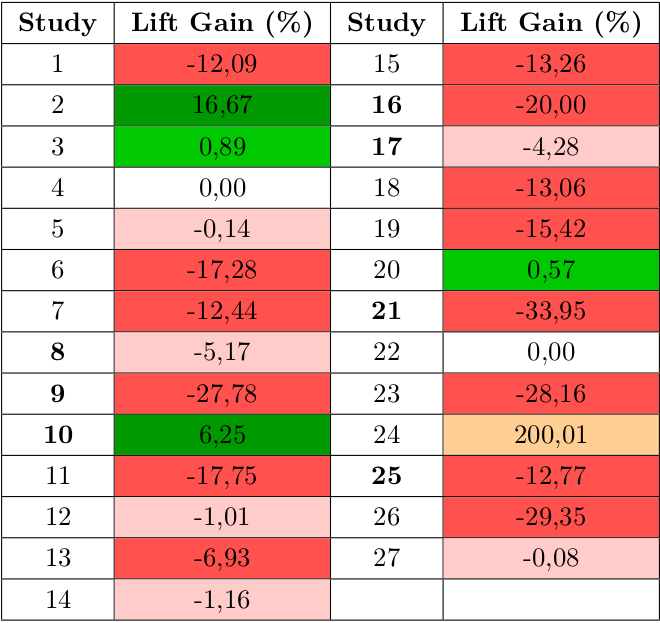
\includegraphics[width=.6\linewidth]{fig/ch4-table-exp-i.png}
        \caption{Summary of the first-decile lift gains for Experiment \nameExperimentI}
    \end{figure}
\end{frame}

%%

\begin{frame}{Results - \fullNameExperimentI{}}
    \begin{figure}
       \centering
       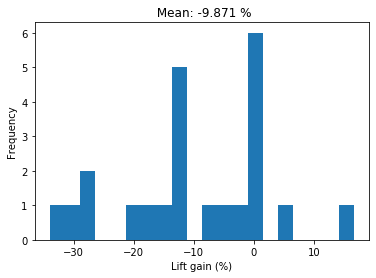
\includegraphics[width=.8\linewidth]{fig/ch4-lift-hist-plot-exp-i.png}
       \caption{Histogram plot of the studies' lift gain for experiment \nameExperimentI{}.}
       \label{fig:lift-hist-plot-exp-i}
    \end{figure}
\end{frame}

%%

\begin{frame}{Results - \fullNameExperimentII{}} \pause
    \begin{figure}
        \centering
        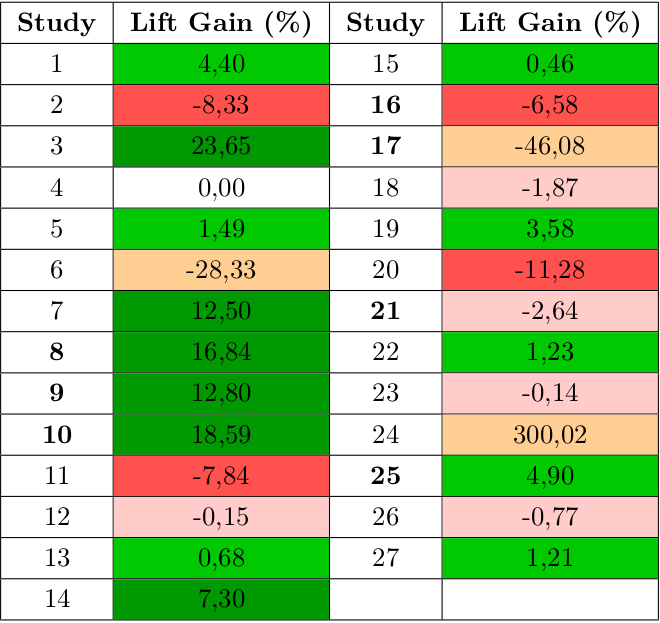
\includegraphics[width=.6\linewidth]{fig/ch4-table-exp-ii.png}
        \caption{Summary of the first-decile lift gains for Experiment \nameExperimentII}
    \end{figure}
\end{frame}

%%

\begin{frame}{Results - \fullNameExperimentII{}}
    \begin{figure}
       \centering
       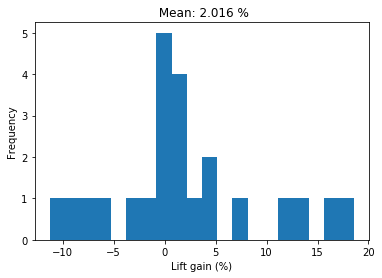
\includegraphics[width=.8\linewidth]{fig/ch4-lift-hist-plot-exp-ii.png}
       \caption{Histogram plot of the studies' lift gain for experiment \nameExperimentII{}.}
       \label{fig:lift-hist-plot-exp-ii}
    \end{figure}
\end{frame}

%%

\begin{frame}{Results - Similarity distributions} \pause
    \textbf<7->{No change} \\  \pause
    \vspace{0.5cm}
    Marginal gain \\ \pause
    \vspace{0.5cm}
    Considerable gain \\ \pause
    \vspace{0.5cm}
    Outliers \\ \pause
    \vspace{0.5cm}
    Heterogeneous portfolio \\ \pause
    \vspace{0.5cm}
    Other relevant 
\end{frame}

%%

\begin{frame}{Results - Similarity distributions - No change}
    \begin{figure}
       \centering
       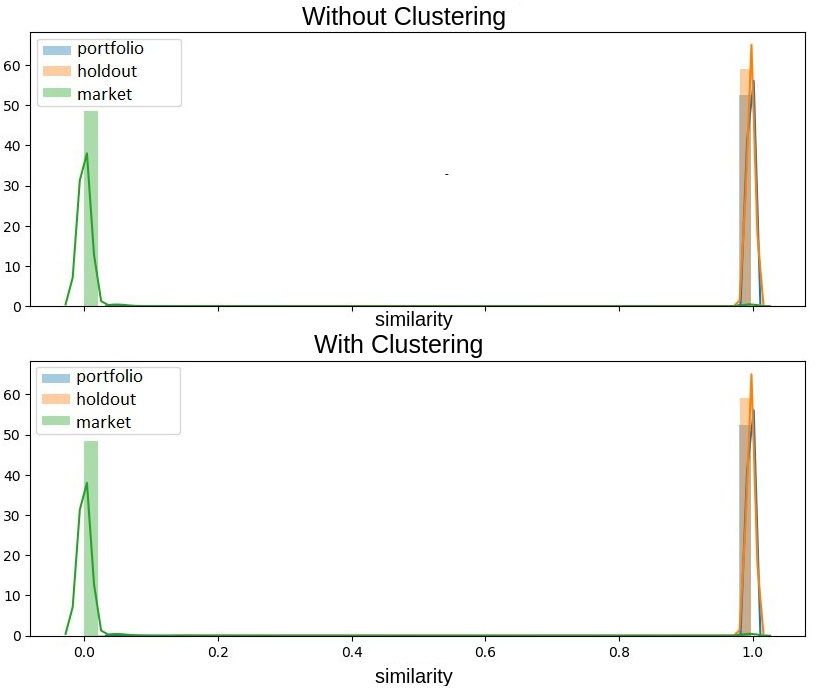
\includegraphics[width=8cm]{fig/ch4-study-4-comparsion-exp-i.png}
       \caption{Similarity distribution plot for Study 4 in experiment \nameExperimentI{}.}
    \end{figure}
\end{frame}

%%

\begin{frame}{Results - Similarity distributions - No change}
    \begin{figure}
        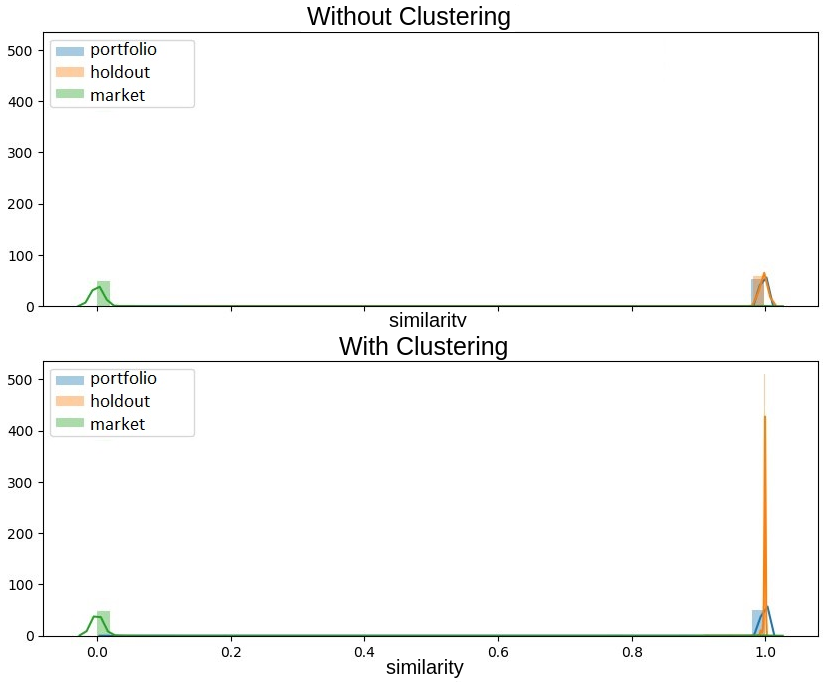
\includegraphics[width=8cm]{fig/ch4-study-4-comparsion-exp-ii.png} 
        \caption{Similarity distribution plot for Study 4 in experiment \nameExperimentII{}.}
    \end{figure}
\end{frame}

%%

\begin{frame}{Results - Similarity distributions - No change}
    \begin{figure}
       \centering
       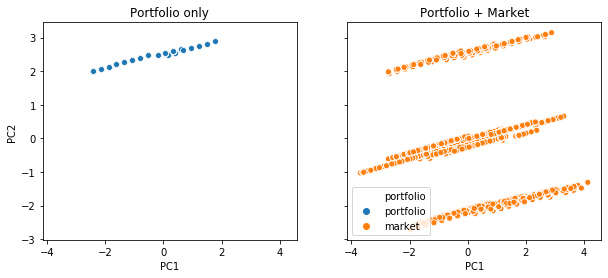
\includegraphics[width=\linewidth]{fig/ch4-study-4-pca-plot.png}
       \caption{PCA plot for Study 4.}
    \end{figure}
\end{frame}

%%

\begin{frame}{Results - Similarity distributions - No change}
    \begin{figure}
       \centering
       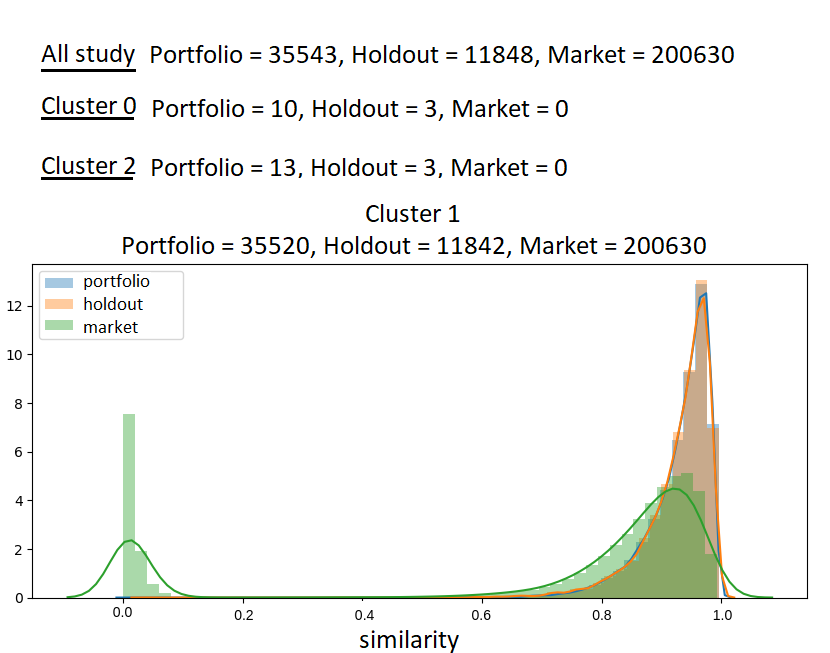
\includegraphics[width=8cm]{fig/ch4-study-22-clusters-simi-plot.png}
       \caption{Similarity distribution plot for the clusters' runs of Study 22 in experiment \nameExperimentI{}.}
    \end{figure}
\end{frame}

%%

\begin{frame}{Results - Similarity distributions}
    No change \\ 
    \vspace{0.5cm}
    \textbf{Marginal gain} \\
    \vspace{0.5cm}
    Considerable gain \\
    \vspace{0.5cm}
    Outliers \\
    \vspace{0.5cm}
    Heterogeneous portfolio \\
    \vspace{0.5cm}
    Other relevant 
\end{frame}

%%

\begin{frame}{Results - Similarity distributions - Marginal gain}
    \begin{figure}
        \centering
        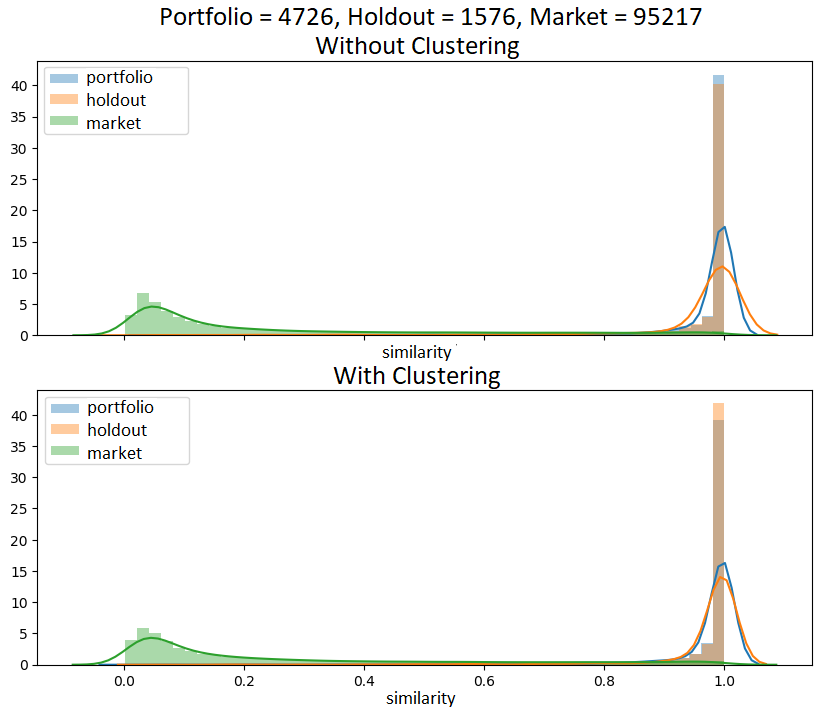
\includegraphics[width=8cm]{fig/ch4-study-5-marginal-increase-exp-2.png}
        \caption{Similarity distribution plot for Study 5 in experiment \nameExperimentII{}.}
    \end{figure}
\end{frame}

%%

\begin{frame}{Results - Similarity distributions - Marginal gain}
    \begin{figure}
        \centering
        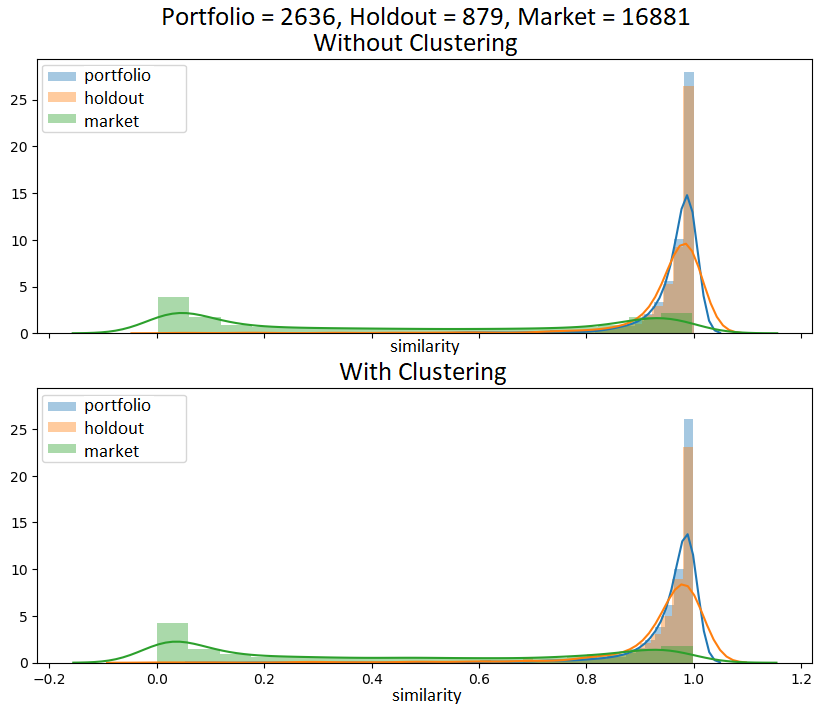
\includegraphics[width=8cm]{fig/ch4-study-12-marginal-decrease-exp-1.png}
        \caption{Similarity distribution plot for Study 12 in experiment \nameExperimentI{}.}
    \end{figure}
\end{frame}

%%

\begin{frame}{Results - Similarity distributions}
    No change \\ 
    \vspace{0.5cm}
    Marginal gain \\
    \vspace{0.5cm}
    \textbf{Considerable gain} \\
    \vspace{0.5cm}
    Outliers \\
    \vspace{0.5cm}
    Heterogeneous portfolio \\
    \vspace{0.5cm}
    Other relevant 
\end{frame}

%%

\begin{frame}{Results - Similarity distributions - Considerable gain}
    \begin{figure}
       \centering
       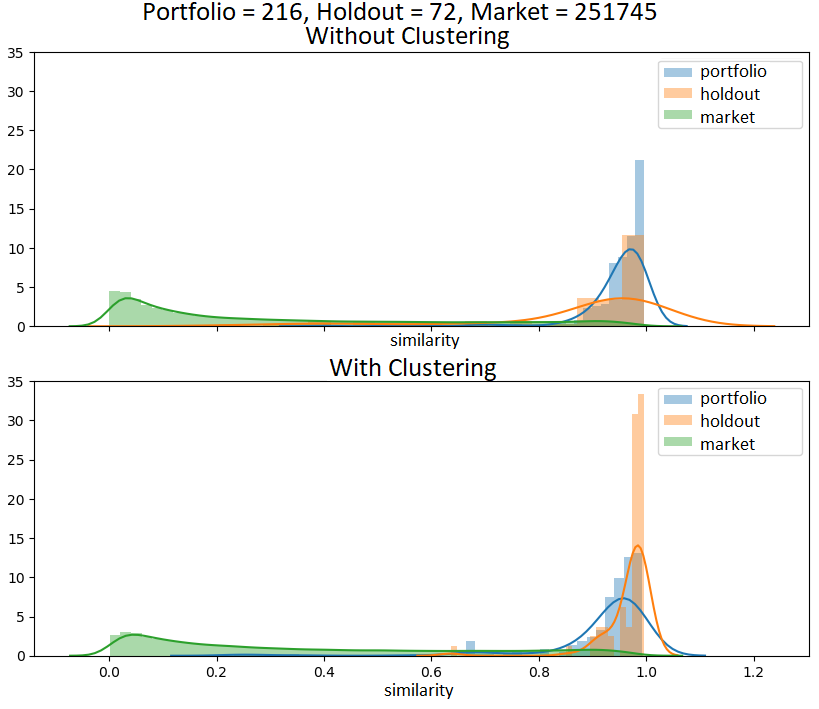
\includegraphics[width=8cm]{fig/ch4-study-8-considerable-increase-exp-2.png}
       \caption{Similarity distribution plot for Study 8 in experiment \nameExperimentII{}.}
    \end{figure}
\end{frame}

%%

\begin{frame}{Results - Similarity distributions - Considerable gain}
    \begin{figure}
       \centering
       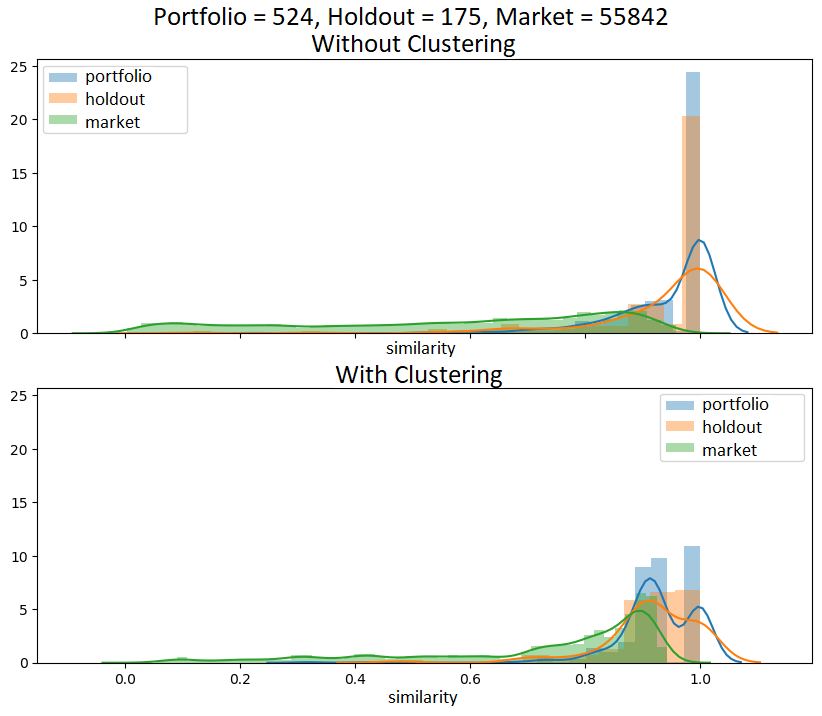
\includegraphics[width=8cm]{fig/ch4-study-9-considerable-decrease-exp-1.png}
       \caption{Similarity distribution plot for Study 9 in experiment \nameExperimentI{}.}
    \end{figure}
\end{frame}

%%

\begin{frame}{Results - Similarity distributions}
    No change \\ 
    \vspace{0.5cm}
    Marginal gain \\
    \vspace{0.5cm}
    Considerable gain \\
    \vspace{0.5cm}
    \textbf{Outliers} \\
    \vspace{0.5cm}
    Heterogeneous portfolio \\
    \vspace{0.5cm}
    Other relevant 
\end{frame}

%%

\begin{frame}{Results - Similarity distributions - Outliers}
    \begin{figure}
       \centering
       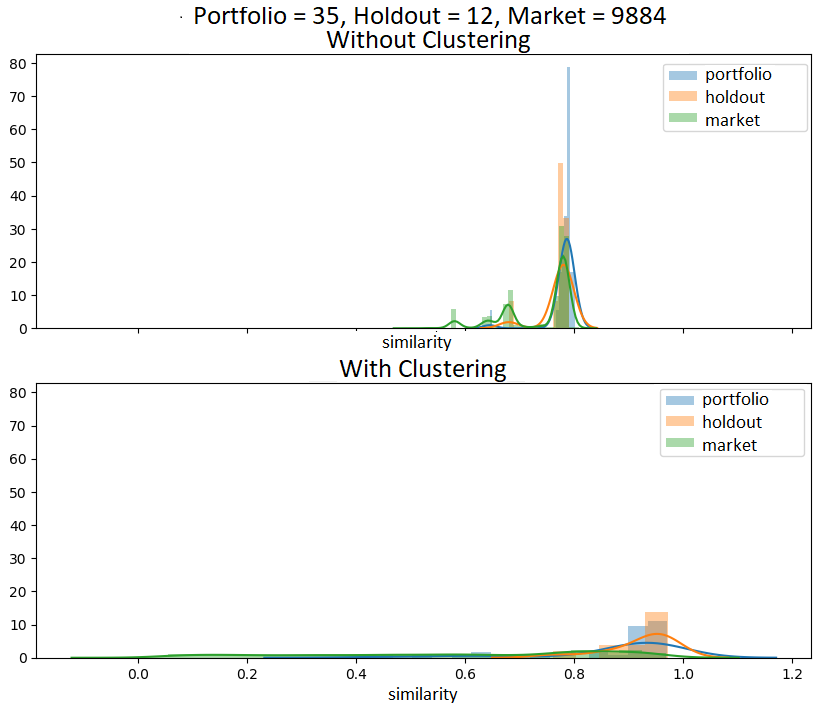
\includegraphics[width=8cm]{fig/ch4-outlier-study-24-exp-2.png}
       \caption{Similarity distribution plot for Study 24 in experiment \nameExperimentII{}.}
    \end{figure}
\end{frame}

%%

\begin{frame}{Results - Similarity distributions - Outliers}
    \begin{figure}
       \centering
       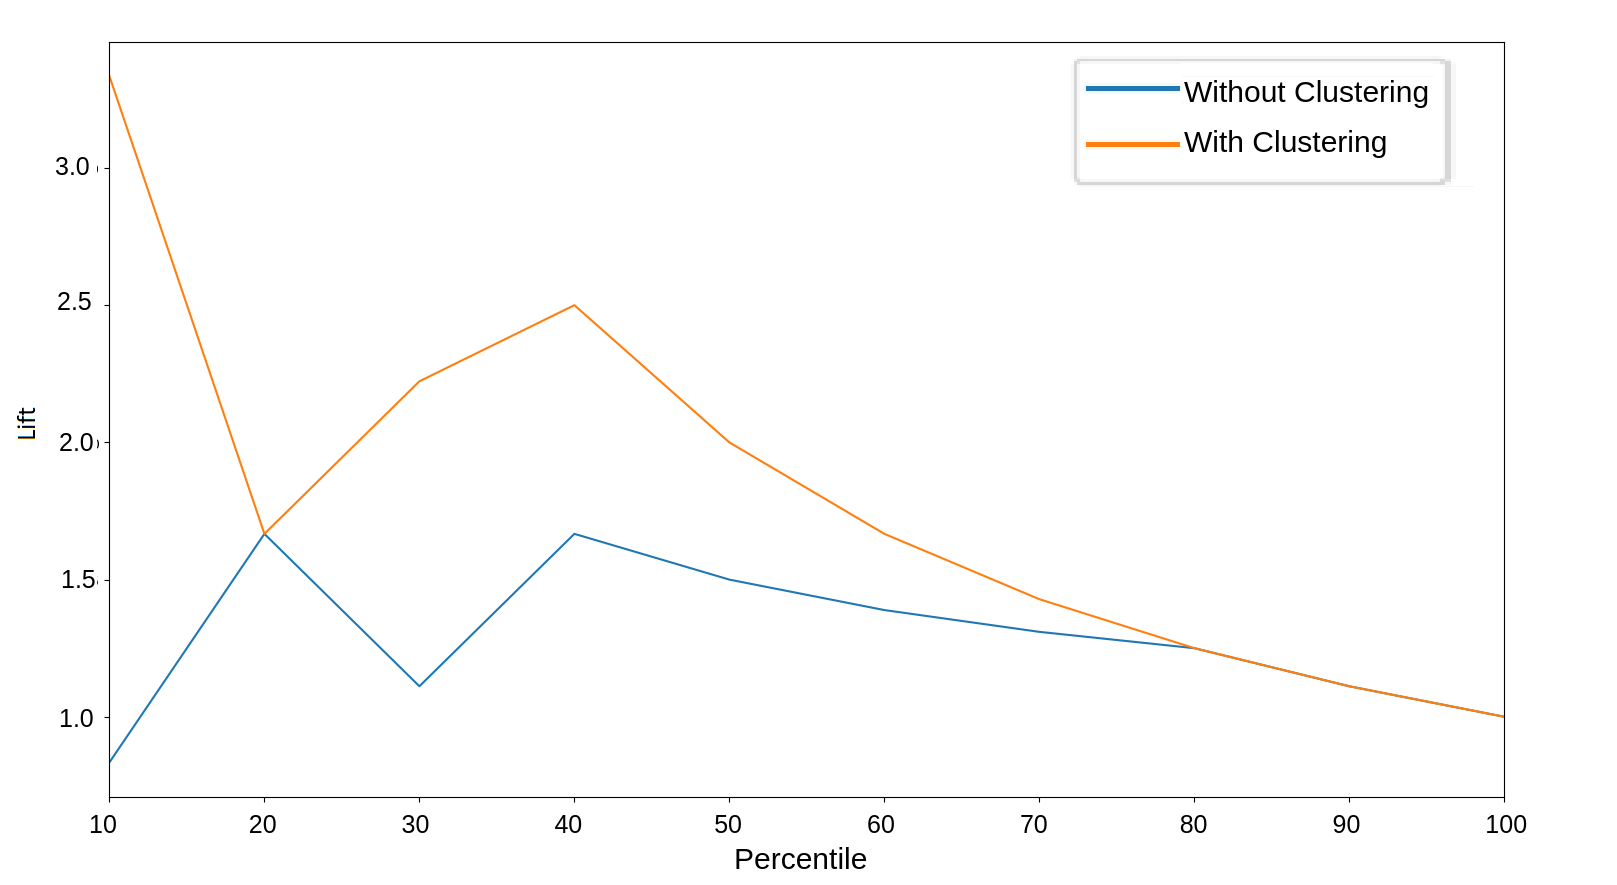
\includegraphics[width=\linewidth]{fig/ch4-outlier-study-24-lift-exp-2.png}
       \caption{Lift plot for Study 24 in experiment \nameExperimentII{}}
    \end{figure}
\end{frame}

%%

\begin{frame}{Results - Similarity distributions}
    No change \\ 
    \vspace{0.5cm}
    Marginal gain \\
    \vspace{0.5cm}
    Considerable gain \\
    \vspace{0.5cm}
    Outliers \\
    \vspace{0.5cm}
    \textbf{Heterogeneous portfolio} \\
    \vspace{0.5cm}
    Other relevant 
\end{frame}

%%

\begin{frame}{Results - Similarity distributions - Heterogeneous portfolio}
    \begin{figure}
       \centering
       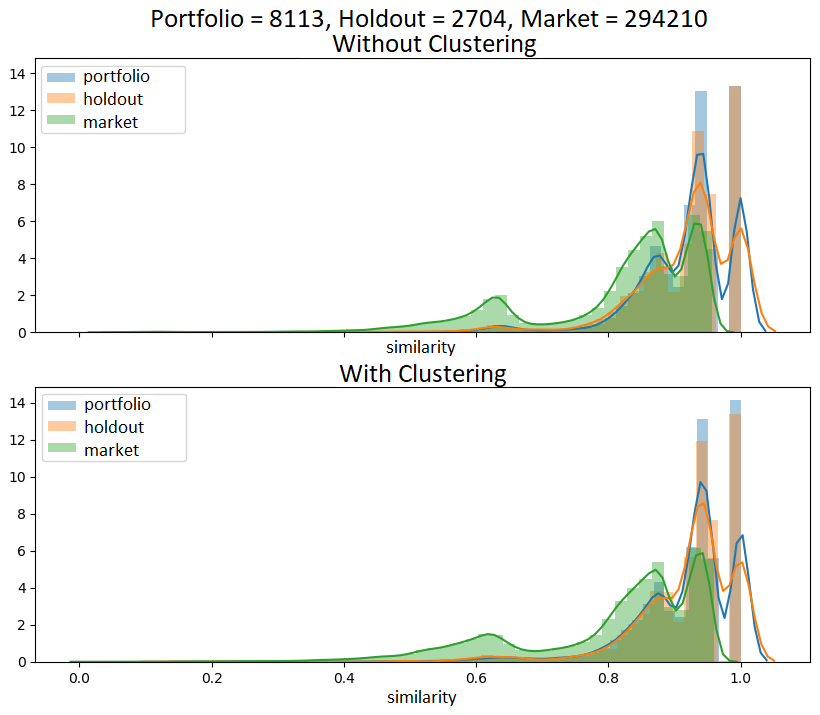
\includegraphics[width=8cm]{fig/ch4-bump-study-25.png}
       \caption{Similarity distribution plot for Study 25 in experiment \nameExperimentII{}.}
    \end{figure}
\end{frame}

%%

\begin{frame}{Results - Similarity distributions - Heterogeneous portfolio}
    \begin{figure}
       \centering
       \caption{PCA plot with portfolio and market data for Study 25.}
       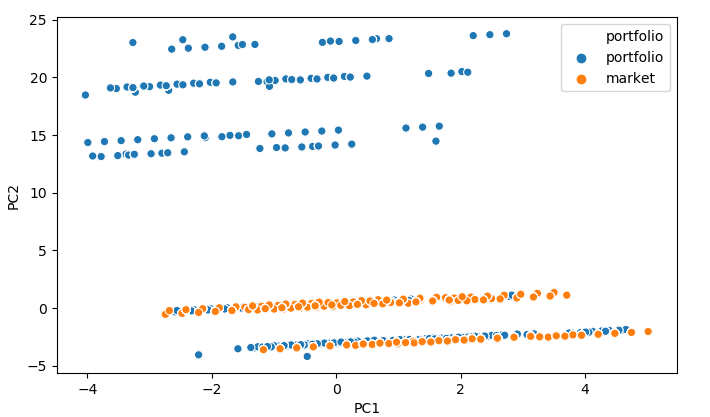
\includegraphics[width=8cm]{fig/ch4-study-25-pca.png}
    \end{figure}
\end{frame}

%%

\begin{frame}{Results - Similarity distributions - Heterogeneous portfolio}
    \begin{figure}
       \centering
       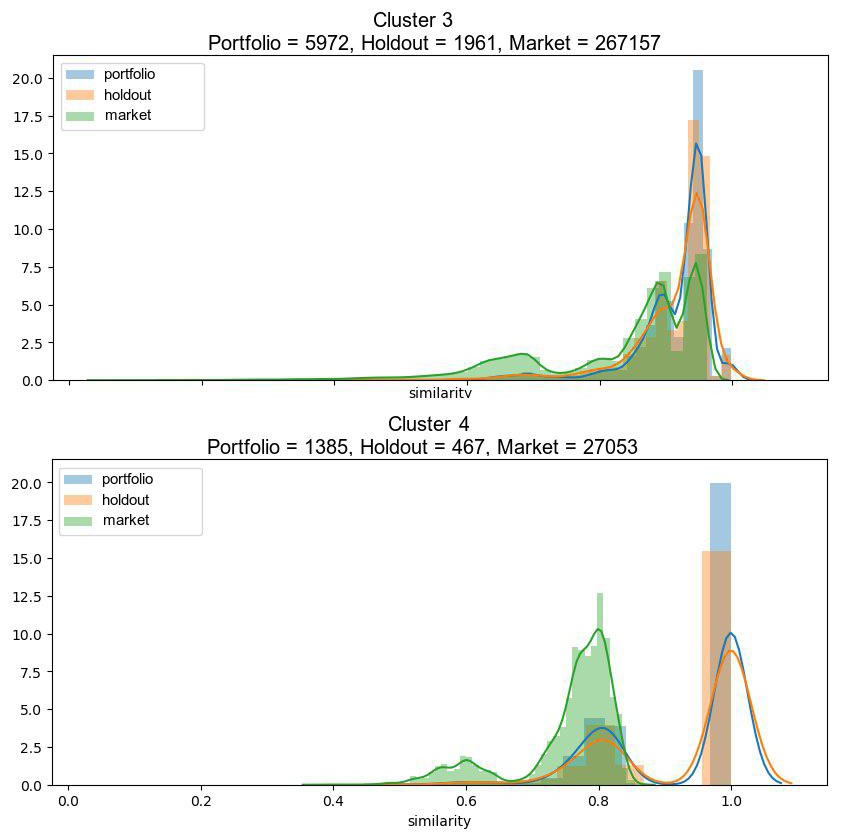
\includegraphics[width=7cm]{fig/ch4-study-25-clusters-simi-plot.png}
       \caption{Clusters' similarity distributions plots for Study 25 in experiment \nameExperimentI{}.}
    \end{figure}
\end{frame}

%%

\begin{frame}{Results - Similarity distributions}
    No change \\ 
    \vspace{0.5cm}
    Marginal gain \\
    \vspace{0.5cm}
    Considerable gain \\
    \vspace{0.5cm}
    Outliers \\
    \vspace{0.5cm}
    Heterogeneous portfolio \\
    \vspace{0.5cm}
    \textbf{Other relevant} 
\end{frame}

%%

\begin{frame}{Results - Similarity distributions - Other relevant}
    \begin{figure}
       \centering
       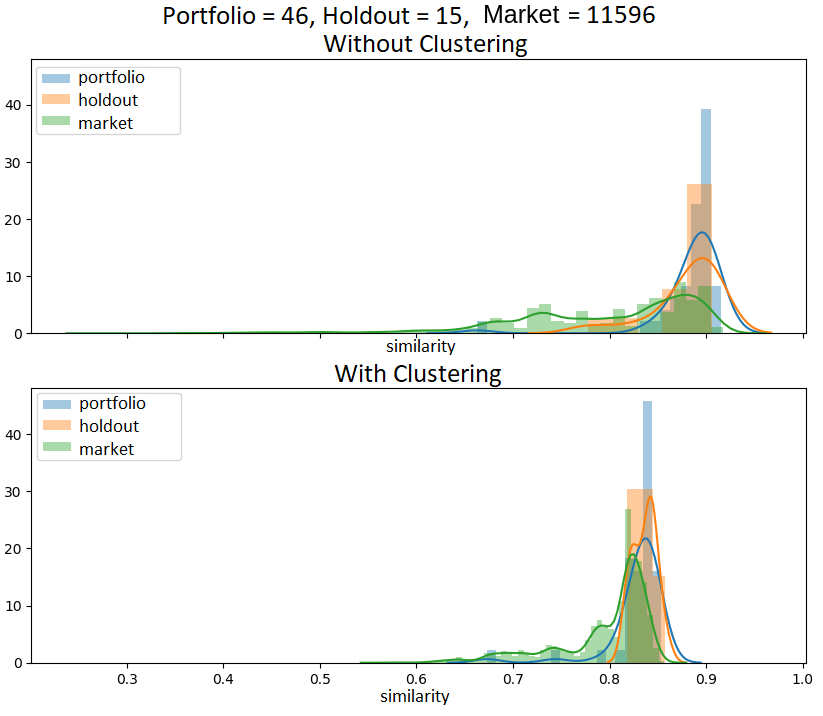
\includegraphics[width=8cm]{fig/ch4-worth-mentioning-study-7.png}
       \caption{Similarity distribution plot for Study 7 in experiment \nameExperimentII{}.}
       \label{fig:worth-mentioning-study-7}
    \end{figure}
\end{frame}

%%

\begin{frame}{Results - Re-run \fullNameExperimentII{}} \pause
    KMeans \\
    \vspace{0.5cm}
    Gaussian Mixture \\
    \vspace{0.5cm}
    Bayesian Gaussian Mixture
\end{frame}

%%

\begin{frame}{Results - Re-run \fullNameExperimentII{}}
    \begin{figure}
        \centering
        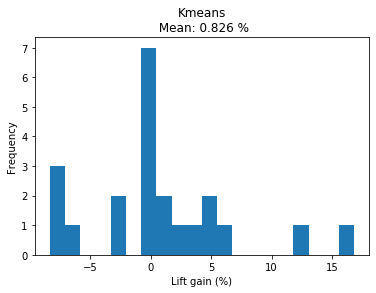
\includegraphics[width=.75\linewidth]{fig/ch4-kmeans_lift_gain_hist.png}
        \caption{Histogram of lift gains for KMeans.}
    \end{figure}
\end{frame}

%%

\begin{frame}{Results - Re-run \fullNameExperimentII{}}
    \begin{figure}
        \centering
        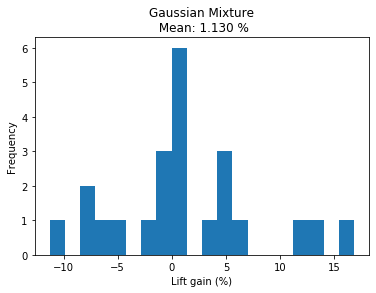
\includegraphics[width=.75\linewidth]{fig/ch4-gmm_lift_gain_hist.png}
        \caption{Histogram of lift gains for Gaussian Mixture.}
    \end{figure}
\end{frame}

%%

\begin{frame}{Results - Re-run \fullNameExperimentII{}}
    \begin{figure}
        \centering
        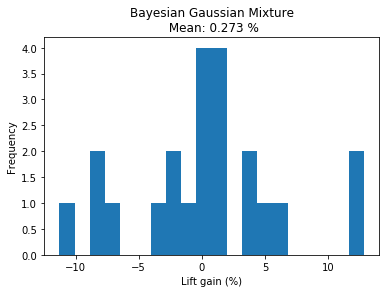
\includegraphics[width=.75\linewidth]{fig/ch4-bgm_lift_gain_hist.png}
        \caption{Histogram of lift gains for Bayesian Gaussian Mixture.}
    \end{figure}
\end{frame}